% CS 455, SP'22 Software Test Plan
% Software test plan template based on the template from
% https://tex.stackexchange.com/questions/42602/software-requirements-specification-with-latex
% and influenced by the IEEE 829-2008 standard
%
\documentclass[letterpaper,12pt,oneside,listof=totoc]{scrreprt}
\usepackage{listings}
\usepackage{underscore}
\usepackage{graphicx}
\usepackage{multicol}
\usepackage[bookmarks=true]{hyperref}
\hypersetup{
    bookmarks=false,                                % show bookmarks bar
    pdftitle={Software Test Plan}, % title
%    pdfauthor={Yiannis Lazarides},                  % author
%    pdfsubject={TeX and LaTeX},                     % subject of the document
%    pdfkeywords={TeX, LaTeX, graphics, images},     % list of keywords
    colorlinks=true,                                % false: boxed links; true: colored links
    linkcolor=blue,                                 % color of internal links
    citecolor=black,                                % color of links to bibliography
    filecolor=black,                                % color of file links
    urlcolor=purple,                                % color of external links
    linktoc=page                                    % only page is linked
}%
\def\myversion{1.0 }

\date{\today}
\author{} % suppress warning, do not fill this in
\begin{document}

% we don't use \maketitle because we overide the default title page here
\begin{titlepage}
\flushright
\rule{\textwidth}{5pt}\vskip1cm
\Huge{SOFTWARE TEST PLAN}\\
\vspace{1.5cm}
for\\
\vspace{1.5cm}
Materials Ordering System\\
\vspace{1.5cm}
\LARGE{Release 1.0\\}
\vspace{1.5cm}
\LARGE{Version \myversion approved\\}
\vspace{1.5cm}
Prepared by Agent Team\\
\vfill
\rule{\textwidth}{5pt}
\end{titlepage}

\tableofcontents
% this will be automatically created from chapters, sections, and subsections

\listoffigures
% this will be automatically created from the figure environment

\listoftables
% this will be automatically created from the table environment

\chapter*{Revision History}
% Update this table for each revision of the requirements
% Add the new content followed by a \hline

\begin{tabular}{| c | p{0.60\textwidth} | p{0.30\textwidth} |}
\hline
Date     & Description   & Revised by \\
\hline
04/11/22 & Initial draft & Agent Team \\
\hline
\end{tabular}

\chapter{INTRODUCTION}

%This section introduces the following subsections, identifies the purpose of this document, and places this document in context with respect to the overall project and other documents.
This document provides test plan for Agents. Test plan include ensure Agents is running in the correct environment. Agents will test for fault data collected, and make sure data are in JSON format. Agents will test to ensure if data can be sent successful over network.



\section{Scope}

%Provide a description and scope of the software and explain the goals, objectives and benefits of your project. This is the executive summary of the system and your team's subsystem.

The goal of the Agent is to collect system data on the device that it's monitoring. A unique ID will generator by the Agent, and all the data collected (including the ID) will be sending to the Engine every minuet in JSON format. 


\section{References}

List any documents, if any, which were used as sources of information. For example, IEEE 829-2008.




\section{System Overview}

%Provide an overview of this document and its organization.
This document(STP) begin with the overall purpose(test plan). STP contain all the references used for testing and the layout of this document. The main focus of STP are the master test plan with 4 different levels. STP end with general overview of the test plan for Agent, that is Quality assurance, Metrics, Test coverage. 


\section{Organization}

%Describe how the testing process is related to the other project processes such as requirements, management, design, quality assurance, and configuration management. Include lines of communication in the testing organization and show how they relate to the overall project organization. You may use an org chart.

Test plan for Agent will follow the design from Software Design Document(SDD), and follow the requirements form the Software Requirements Specification (SRS). Configuration management will be done by using Git. 

Testing requirements include: 
\begin{enumerate}

\item  Make sure data can be collect from both MS-Windows and Ubuntu Linux
systems. 
    \begin{itemize}
    \item It will be done by running program in both system and fixing errors. To do this we will use a Linux OS called Raspbian to test it. For MS-Windows we will use a Windows 10 System to test it.
    \end{itemize}
    
\item  Make sure the correct data from the system is being collected. 
    \begin{itemize}
    \item To do this we will have the system manager on the screen to see if we are receiving the same data.
    \end{itemize}
    
\item  Data must sent over local host. 
    \begin{itemize}
    \item Test using Netcat commands over local host.
    \end{itemize}
    
\item  Data must sent over open network. 
    \begin{itemize}
    \item Test using Netcat commands over the internet.
    \end{itemize}

\end{enumerate}

\newpage
\section{Master test schedule}

%Describe how the testing tasks are incorporated into the overall software development lifecycle. List any milestones and summarize the overall testing schedule.

Table~\ref{Schedule} describes the test plan schedule.

\begin {table}[h!]
\begin{tabular}{|p{.1\textwidth} | p{.1\textwidth}|p{.1\textwidth}| p{.7\textwidth }|}
\hline
\textbf {Item} & \textbf{Date} &\textbf{Level} &\textbf{Detail}\\
    \hline
    1 & 4/12 & 4 & Running Agent in different environment \\
    \hline
    2 & 4/12 & 3 & Check for data collect(Ex. CPU usage must be less than 100 and great than or equal to 0) \\
    \hline
    3 & 4/14 & 3 & Data must be in JSON format \\
    \hline
    4 & 4/14 & 4 & Data must be able to sent to Engine using network \\
    \hline
    \end{tabular}
    \caption{Test Plan Schedule}
    \label{Schedule}
\end {table}

\section{Software integrity levels}

\begin{table}
\centering

\begin{tabular}{|c|c|}
\hline
Integrity level & \\
identifier      & Description \\
\hline
Level 4         & Catastrophic \\
Level 3         & Critical \\
Level 2         & Marginal \\
Level 1         & Negligible \\
\hline
\end{tabular}
\label{sils}
\caption{Software integrity levels}
\end{table}

An integrity level scheme is used to provide a structured classification mechanism for denoting overall breadth and depth of testing for each testable portion of the system. Integrity levels may be applied to a variety of items including requirements, functions, classes or collections of functions, modules, subsystems, or whole systems. Table~\ref{sils} shows the software integrity level scheme that will be used to denote the minimum required testing tasks for a testable unit. Each testable unit will be assigned one of the four integrity levels shown. The required amount of testing is dictated by the level with Level 4 indicating exhaustive testing should be performed to ensure correctness and Level 1 testing indicating that basic functional is required. The scheme is drawn from the IEEE Standard for Software and System Test Document (IEEE 829-2008).

\section{Resources summary}

%Give a list or summary of the resources required to perform testing.
Resources need for Agent test plan will be machines that are in different operating environments. 


\section{Responsibilities}

%Describe who is responsible for testing (which organizational entity) and their test-related responsibilities. You may use your org chart and refer to it.

Devin and Jatin will be test engineer for Agent. Those engineer will follow the test plan and collect data/errors form the testing result. 

\section{Tools, techniques, methods, and metrics}

%Describe the documents, hardware, software, test tools, methods, and test environment to be used in the test process.

The test environment for Agent will be on a Windows 10 machine and UNIX based Machine. Agents will be build using Python and data collection will be using Python build in modules list below. 
\begin{multicols}{2}
\begin{itemize}
 \item os 
 \item psutil 
 \item json
 \item uuid 
 \item time
 \item network
 \item datetime 
 \end{itemize}
\end{multicols}





\chapter{MASTER TEST PLAN}

\section{Level 4 test }
Network Connection.
%List the test items that are rated Level 4. All of the following subsections will be repeated for levels 3, 2, and 1 in subsequent sections.

\subsection{Traceability matrix}

Show each test case and its source (requirement's ID). The matrix links each requirements with one or more test cases. This may be a table.

\subsection{Approach}
\begin{itemize}
    \item Network Connection - Black Box testing using Pytest to have the test input data into the network and then send it to the local host network as a test to see if we can send data. We will check for whether the JSON was the same pre and post sending.
\end{itemize}
\endlist

NOTE: This section may be combined with the traceability matrix into a single table.

\subsection{Pass/Fail criteria}

Level 4 tests must complete the sending of data and have the matching JSON be sent to the local host used for testing. If the JSON does not match exactly then the test has failed and will be reported by Pytest.

%\section{Suspension/Resumption criteria}
%  ** N/A **
% This section describe when test may be suspended and what must be done when tests are resumed.

\subsection{Test deliverables}

\begin{figure}
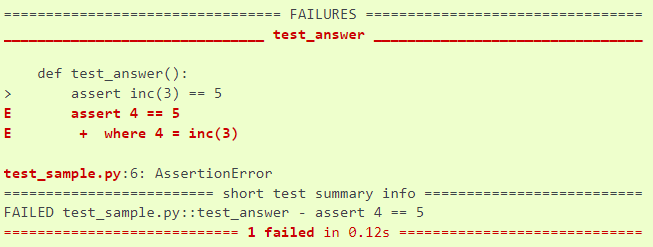
\includegraphics[width=15cm]{deliverable.png}
  \caption{\label{fig:module} Pytest Test Deliverable }
\end{figure}
At the beginning of each run of the Agent there will be a Pytest check. This Pytest check will print a deliverable as seen in figure 2.1. This deliverable will be taken and recorded by the testing team and then logged to be fixed by the software team. We will look to see if this is a common problem among most agents, report it and get it fixed.

% And now the level 3 test section
\section{Level 3 test plan}
Data Correctness.
\subsection{Traceability matrix}

\subsection{Approach}
Data Correctness - Black Box testing using Pytest. We will use the assert methos inside Pytest to test weither the data is coming from the machine correctly. If the data is greater than zero and less than one-hundred then we are getting the correct data from the machine and the test will pass.
\subsection{Pass/Fail criteria}
The data must be between zero and one-hundred for the data to pass. If the data is under or over that then the test will fail.
\subsection{Test deliverables}
The deliverables will be just like the level four deliverables. The Pytest deliverable.
% And now the level 2 test section
\section{Level 2 test plan}
N/A
\subsection{Traceability matrix}
N/A
\subsection{Approach}
N/A
\subsection{Pass/Fail criteria}
N/A
\subsection{Test deliverables}
N/A
% And now the level 1 test section
\section{Level 1 test plan}
N/A
\subsection{Traceability matrix}
N/A
\subsection{Approach}
N/A
\subsection{Pass/Fail criteria}
N/A
\subsection{Test deliverables}
N/A


\chapter{GENERAL}

\section{Quality assurance}

Quality assurance will be done through software performance testing. Through data correctness checking and Black Box testing with Pytest, the quality of the software will be up to standard.

\section{Metrics}

Level 1: Data Correctness and error logging if connection to the driver fails.
Level 2: Function-oriented metrics to measure the function points and errors per function points. 

Level 3: Error logging if connection to the engine fails.


\section{Test coverage}

This is how many lines of our code is being tested. Test coverage will be done by using the Pytest features stated earlier.

\end{document}
